\documentclass[12pt,a4paper]{article}
\usepackage[utf8]{inputenc}
\usepackage[T1]{fontenc}
\usepackage{german}
\usepackage{microtype}

\usepackage{amsmath, amssymb, amsthm}
\usepackage{physics}
\usepackage{siunitx}
\usepackage{tikz}
\usepackage{tikz-3dplot}
\usetikzlibrary{arrows.meta, decorations.pathmorphing, decorations.markings,
                patterns, calc, positioning, shapes.geometric, angles, quotes,
                decorations.pathreplacing, backgrounds, hobby}
\usepackage{pgfplots}
\pgfplotsset{compat=1.18}
\usepackage{booktabs}
\usepackage{array}
\usepackage{multirow}
\usepackage{geometry}
\usepackage{graphicx}
\usepackage{xcolor}
\usepackage{hyperref}
\usepackage{cleveref}
\usepackage{float}
\usepackage{caption}
\usepackage{subcaption}
\usepackage{enumitem}
\usepackage{fancyhdr}
\usepackage{titlesec}

\geometry{
  a4paper,
  left=2.5cm, right=2.5cm,
  top=3cm, bottom=3cm
}

\definecolor{raumblau}{RGB}{10,40,100}
\definecolor{triebwerkorange}{RGB}{220,100,20}
\definecolor{hellgrau}{RGB}{240,240,245}
\definecolor{dunkelgrau}{RGB}{80,80,90}
\definecolor{flammenrot}{RGB}{200,50,20}
\definecolor{exhaust}{RGB}{180,200,230}

\hypersetup{
  colorlinks=true,
  linkcolor=raumblau,
  citecolor=raumblau,
  urlcolor=raumblau,
  pdftitle={Raketenantriebe in der Raumfahrt},
  pdfauthor={Stephan Epp}
}

\newtheorem{satz}{Satz}[section]
\newtheorem{definition}{Definition}[section]
\newtheorem{herleitung}{Herleitung}[section]

\newcommand{\vek}[1]{\boldsymbol{#1}}
\newcommand{\Isp}{I_{\mathrm{sp}}}
\newcommand{\ve}{v_e}
\newcommand{\mdot}{\dot{m}}
\newcommand{\Dv}{\Delta v}

%-------------------------------------------------------
\title{Raketenantriebe in der Raumfahrt\\[0.4em]
  \large\textit{Formale Grundlagen, Thermodynamik, Antriebskonzepte\\
und Bahnmechanik mit vollst\"{a}ndigen Herleitungen}}
\author{Stephan Epp}
\date{\today}

\begin{document}

\maketitle

\tableofcontents
\newpage

%=======================================================
\section{Einleitung und physikalische Grundlagen}
%=======================================================

Die Raumfahrt steht und fällt mit einer einzigen fundamentalen Frage: \emph{Wie bewegt
man sich in einem Medium fort, das keinen Widerstand bietet?} Der klassische
Kolbenmotor überträgt Kraft auf Boden oder Luft; im Vakuum des Weltraums ist beides
nicht vorhanden. Die Lösung liefert das dritte Newtonsche Axiom in seiner reinsten
Form: \textit{actio} = \textit{reactio}. Jede Masse, die mit hoher Geschwindigkeit
nach hinten ausgestoßen wird, erzeugt einen Impuls nach vorne --- dies ist das
Raketenprinzip.

\subsection{Das Raketenprinzip --- Impulserhaltung}

Betrachten wir eine Rakete der Masse $m(t)$ im massefreien Raum. Im Zeitintervall
$\dd t$ wird eine Treibstoffmasse $|\dd m|$ mit der Ausströmgeschwindigkeit $\ve$
relativ zur Rakete ausgestoßen.

\begin{herleitung}[Raketengrundgleichung (Tsiolkowski)]
\textbf{Impuls zum Zeitpunkt $t$:}
\[
  p(t) = m(t)\,v(t)
\]
\textbf{Impuls zum Zeitpunkt $t + \dd t$:}
\[
  p(t+\dd t) = \underbrace{(m+\dd m)(v+\dd v)}_{\text{Rakete}} +
               \underbrace{(-\dd m)(v - \ve)}_{\text{ausgestoßenes Gas}}
\]
(da $\dd m < 0$ ist $-\dd m > 0$ die ausgestoßene Masse)

\textbf{Impulserhaltung} ($\Delta p_{\text{ext}} = 0$ im kräftefreien Raum):
\begin{align}
  p(t+\dd t) &= p(t) \notag\\
  (m+\dd m)(v+\dd v) + (-\dd m)(v-\ve) &= mv \notag\\
  mv + m\,\dd v + v\,\dd m + \dd m\,\dd v - v\,\dd m + \ve\,\dd m &= mv \notag
\end{align}
Vernachlässigung des Produkts $\dd m\,\dd v$ (Terme zweiter Ordnung):
\[
  \boxed{m\,\dd v = -\ve\,\dd m}
\]
Dies ist die \textbf{Raketengrundgleichung}.
\end{herleitung}

\subsection{Tsiolkowski-Gleichung}

Die Integration der Raketengrundgleichung liefert die berühmte
Tsiolkowski-Gleichung:

\begin{align}
  \int_{v_0}^{v_1} \dd v &= -\ve \int_{m_0}^{m_1} \frac{\dd m}{m} \notag\\
  v_1 - v_0 &= \ve \ln\!\left(\frac{m_0}{m_1}\right)
\end{align}

\begin{satz}[Tsiolkowski-Gleichung]
Das erreichbare Geschwindigkeitsinkrement $\Dv$ einer Rakete im kräftefreien Raum
beträgt:
\[
  \boxed{\Dv = \ve \ln\!\left(\frac{m_0}{m_1}\right) = \ve \ln\!\left(\frac{m_0}{m_0 - m_p}\right)}
\]
wobei $m_0$ die Startmasse, $m_1$ die Endmasse und $m_p = m_0 - m_1$ die
verbrauchte Treibstoffmasse bezeichnet.
\end{satz}

\begin{figure}[H]
\centering
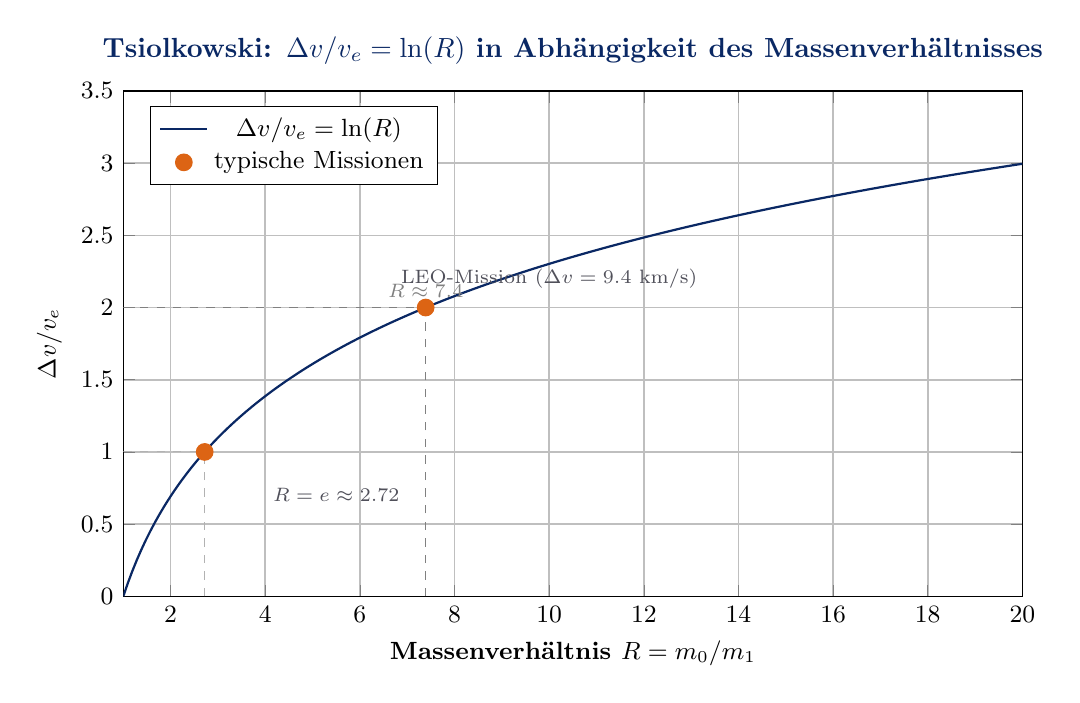
\begin{tikzpicture}[scale=1.0]
\begin{axis}[
  width=13cm, height=8cm,
  xlabel={Massenverhältnis $R = m_0/m_1$},
  ylabel={$\Dv / \ve$},
  xmin=1, xmax=20,
  ymin=0, ymax=3.5,
  grid=both,
  grid style={line width=0.3pt, draw=gray!30},
  major grid style={line width=0.6pt, draw=gray!50},
  tick label style={font=\small},
  label style={font=\small\bfseries},
  title style={font=\normalsize\bfseries\color{raumblau}},
  title={Tsiolkowski: $\Dv/\ve = \ln(R)$ in Abhängigkeit des Massenverhältnisses},
  legend pos=north west,
  legend style={font=\small},
]
\addplot[thick, color=raumblau, domain=1:20, samples=200] {ln(x)};
\addlegendentry{$\Dv/\ve = \ln(R)$}

% Markierungen typischer Missionen
\addplot[only marks, mark=*, mark size=3pt, color=triebwerkorange]
  coordinates {(7.39, 2.0) (2.72, 1.0) (20.09, 3.0)};
\addlegendentry{typische Missionen}

\draw[dashed, gray] (axis cs:7.39,0) -- (axis cs:7.39,2.0)
  node[above, font=\scriptsize, rotate=0] {$R\approx 7.4$};
\draw[dashed, gray] (axis cs:1,2.0) -- (axis cs:7.39,2.0);
\node[font=\scriptsize, color=dunkelgrau] at (axis cs:10,2.2)
  {LEO-Mission ($\Dv=9.4$ km/s)};

\draw[dashed, gray!60] (axis cs:2.72,0) -- (axis cs:2.72,1.0);
\draw[dashed, gray!60] (axis cs:1,1.0) -- (axis cs:2.72,1.0);
\node[font=\scriptsize, color=dunkelgrau] at (axis cs:5.5,0.7)
  {$R=e \approx 2.72$};
\end{axis}
\end{tikzpicture}
\caption{Tsiolkowski-Diagramm: normiertes Geschwindigkeitsinkrement als Funktion
des Massenverhältnisses. Ein $\Dv$ von $\SI{9.4}{km/s}$ (niedrige Erdumlaufbahn)
erfordert bei $\ve = \SI{4.4}{km/s}$ (kryogenes $\mathrm{H_2/O_2}$-Triebwerk)
ein Massenverhältnis von etwa 8.}
\label{fig:tsiol}
\end{figure}

%=======================================================
\section{Thermodynamische Grundlagen des Raketentriebwerks}
%=======================================================

\subsection{De-Laval-Düse und isentrope Strömung}

Das Herzstück jedes chemischen Raketentriebwerks ist die \emph{konvergent-divergente
Lavaldüse}. Sie wandelt die thermische und chemische Energie des Treibgases in
gerichtete kinetische Energie um.

\begin{figure}[H]
\centering
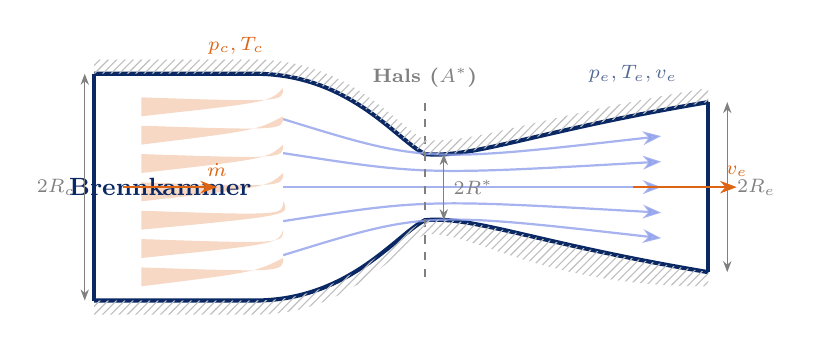
\begin{tikzpicture}[scale=1.2]
  % Düsenkontur (Meridianschnitt)
  \def\Rc{1.2}   % Radius Brennkammer
  \def\Rt{0.35}  % Radius Engstelle (Hals)
  \def\Re{0.9}   % Radius Auslass

  % Obere Kontur
  \draw[thick, raumblau, line width=1.5pt]
    (-3.5, \Rc) -- (-1.8, \Rc)
    .. controls (-0.8, \Rc) and (-0.3, \Rt+0.15) .. (0, \Rt)
    .. controls (0.5, \Rt-0.05) and (1.2, \Re-0.3) .. (3.0, \Re);

  % Untere Kontur
  \draw[thick, raumblau, line width=1.5pt]
    (-3.5,-\Rc) -- (-1.8,-\Rc)
    .. controls (-0.8,-\Rc) and (-0.3,-\Rt-0.15) .. (0,-\Rt)
    .. controls (0.5,-\Rt+0.05) and (1.2,-\Re+0.3) .. (3.0,-\Re);

  % Abschlusslinien
  \draw[thick, raumblau, line width=1.5pt] (-3.5,-\Rc) -- (-3.5,\Rc);
  \draw[thick, raumblau, line width=1.5pt] (3.0,-\Re) -- (3.0,\Re);

  % Flamme / Verbrennungszone (Brennkammer)
  \foreach \yf in {-0.9,-0.6,-0.3,0,0.3,0.6,0.9} {
    \pgfmathsetmacro{\len}{0.4+rand*0.2}
    \fill[triebwerkorange, opacity=0.25]
      (-3.0,\yf-0.15) .. controls (-2.0+\len,\yf) .. (-1.5,\yf+0.15)
      .. controls (-1.5,\yf) .. (-3.0,\yf+0.05) -- cycle;
  }

  % Strömungslinien im Düsenkanal
  \foreach \y in {-0.8,-0.4,0,0.4,0.8} {
    \pgfmathsetmacro{\ys}{\y/\Rc}
    \draw[-{Stealth}, exhaust!80!blue, line width=0.8pt, opacity=0.8]
      (-1.5, \y*0.9) .. controls (0, \y*\Rt/\Rc*1.1) .. (2.5, \y*\Re/\Rc*0.9);
  }

  % Beschriftungen
  \node[font=\small\bfseries, raumblau] at (-2.8, 0) {Brennkammer};
  \node[font=\small\bfseries, raumblau, rotate=90] at (-3.8, 0) {};

  % Staudrucklinie
  \draw[dashed, gray, line width=0.6pt] (0,-\Rt-0.6) -- (0,\Rt+0.6)
    node[above, font=\scriptsize\bfseries, gray] {Hals ($A^*$)};

  % Dreieckige Pfeile für Strömungsrichtung
  \draw[-{Stealth[length=6pt]}, thick, triebwerkorange]
    (-3.2,0) -- (-2.2,0) node[above, font=\scriptsize] {$\dot{m}$};
  \draw[-{Stealth[length=6pt]}, thick, triebwerkorange]
    (2.2,0) -- (3.3,0) node[above, font=\scriptsize] {$v_e$};

  % Querschnittspfeile
  \draw[{Stealth[length=4pt]}-{Stealth[length=4pt]}, gray]
    (-3.6,-\Rc) -- (-3.6,\Rc) node[midway, left, font=\scriptsize] {$2R_c$};
  \draw[{Stealth[length=4pt]}-{Stealth[length=4pt]}, gray]
    (3.2,-\Re) -- (3.2,\Re) node[midway, right, font=\scriptsize] {$2R_e$};
  \draw[{Stealth[length=4pt]}-{Stealth[length=4pt]}, gray]
    (0.2,-\Rt) -- (0.2,\Rt) node[midway, right, font=\scriptsize] {$2R^*$};

  % Druckpfeil oben
  \node[font=\scriptsize, triebwerkorange] at (-2.0,\Rc+0.3) {$p_c, T_c$};
  \node[font=\scriptsize, raumblau!70] at (2.2,\Re+0.3) {$p_e, T_e, v_e$};

  % Schraffur (Wand)
  \fill[pattern=north east lines, pattern color=gray!50]
    (-3.5,\Rc) -- (-1.8,\Rc)
    .. controls (-0.8,\Rc) and (-0.3,\Rt+0.15) .. (0,\Rt)
    .. controls (0.5,\Rt-0.05) and (1.2,\Re-0.3) .. (3.0,\Re)
    -- (3.0,\Re+0.15) .. controls (1.2,\Re-0.15) and (0.5,\Rt+0.1) .. (0,\Rt+0.15)
    .. controls (-0.3,\Rt+0.3) and (-0.8,\Rc+0.15) .. (-1.8,\Rc+0.15)
    -- (-3.5,\Rc+0.15) -- cycle;
  \fill[pattern=north east lines, pattern color=gray!50]
    (-3.5,-\Rc) -- (-1.8,-\Rc)
    .. controls (-0.8,-\Rc) and (-0.3,-\Rt-0.15) .. (0,-\Rt)
    .. controls (0.5,-\Rt+0.05) and (1.2,-\Re+0.3) .. (3.0,-\Re)
    -- (3.0,-\Re-0.15) .. controls (1.2,-\Re-0.15) and (0.5,-\Rt-0.1) .. (0,-\Rt-0.15)
    .. controls (-0.3,-\Rt-0.3) and (-0.8,-\Rc-0.15) .. (-1.8,-\Rc-0.15)
    -- (-3.5,-\Rc-0.15) -- cycle;
\end{tikzpicture}
\caption{Meridianschnitt einer konvergent-divergenten Lavaldüse. In der Brennkammer
herrschen hoher Druck $p_c$ und hohe Temperatur $T_c$. Am Düsenhals wird Schallgeschwindigkeit
($M=1$) erreicht; im divergenten Teil wird die Strömung überschallartig und $v_e$ maximiert.}
\label{fig:laval}
\end{figure}

\subsection{Isentrope Strömungsbeziehungen}

Für ein ideales Gas mit Isentropenexponent $\gamma$ gelten entlang der Düsenströmung
folgende Beziehungen (isentrop, $\kappa = \gamma$):

\begin{align}
  \frac{T_0}{T} &= 1 + \frac{\gamma-1}{2}M^2
  \label{eq:temp_machzahl}\\[4pt]
  \frac{p_0}{p} &= \left(1 + \frac{\gamma-1}{2}M^2\right)^{\!\gamma/(\gamma-1)}
  \label{eq:druck_machzahl}\\[4pt]
  \frac{\rho_0}{\rho} &= \left(1 + \frac{\gamma-1}{2}M^2\right)^{\!1/(\gamma-1)}
  \label{eq:dichte_machzahl}
\end{align}

Die \textbf{Ausströmgeschwindigkeit} ergibt sich aus dem Energiesatz (Enthalpiegefälle):

\begin{herleitung}[Ideale Ausströmgeschwindigkeit]
Energieerhaltung (stationäre adiabate Strömung):
\[
  h_c + \frac{v_c^2}{2} = h_e + \frac{v_e^2}{2}
\]
Mit $v_c \approx 0$ (Düsenhals-Approx.) und $h = c_p T$:
\[
  c_p T_c = c_p T_e + \frac{v_e^2}{2}
  \quad\Rightarrow\quad
  v_e = \sqrt{2 c_p (T_c - T_e)}
\]
Mit $c_p = \frac{\gamma R}{(\gamma-1)\bar{M}}$ und $T_e/T_c = (p_e/p_c)^{(\gamma-1)/\gamma}$:
\[
  \boxed{v_e = \sqrt{\frac{2\gamma}{\gamma-1}\cdot\frac{R\,T_c}{\bar{M}}
    \left[1 - \left(\frac{p_e}{p_c}\right)^{(\gamma-1)/\gamma}\right]}}
\]
wobei $R = \SI{8.314}{J/(mol\cdot K)}$ die universelle Gaskonstante,
$\bar{M}$ die molare Masse des Treibgases und $T_c$ die Brennkammertemperatur ist.
\end{herleitung}

\subsection{Schubkraft und spezifischer Impuls}

\begin{satz}[Schubkraftgleichung]
Die Schubkraft $F$ eines Raketentriebwerks setzt sich aus Impulsschub und Druckschub zusammen:
\[
  \boxed{F = \mdot\,\ve + (p_e - p_a)\,A_e}
\]
wobei $\mdot$ der Massenfluss, $p_e$ der Austrittsdruck, $p_a$ der Umgebungsdruck
und $A_e$ die Austrittsfläche ist. Optimale Expansion: $p_e = p_a$.
\end{satz}

\begin{definition}[Spezifischer Impuls]
Der spezifische Impuls $\Isp$ ist das Maß für die Treibstoffeffizienz eines Triebwerks:
\[
  \boxed{\Isp = \frac{F}{\mdot\,g_0} = \frac{\ve}{g_0}}
\]
mit $g_0 = \SI{9.80665}{m/s^2}$ (Normfallbeschleunigung). Einheit: Sekunden [s].
\end{definition}

\begin{figure}[H]
\centering
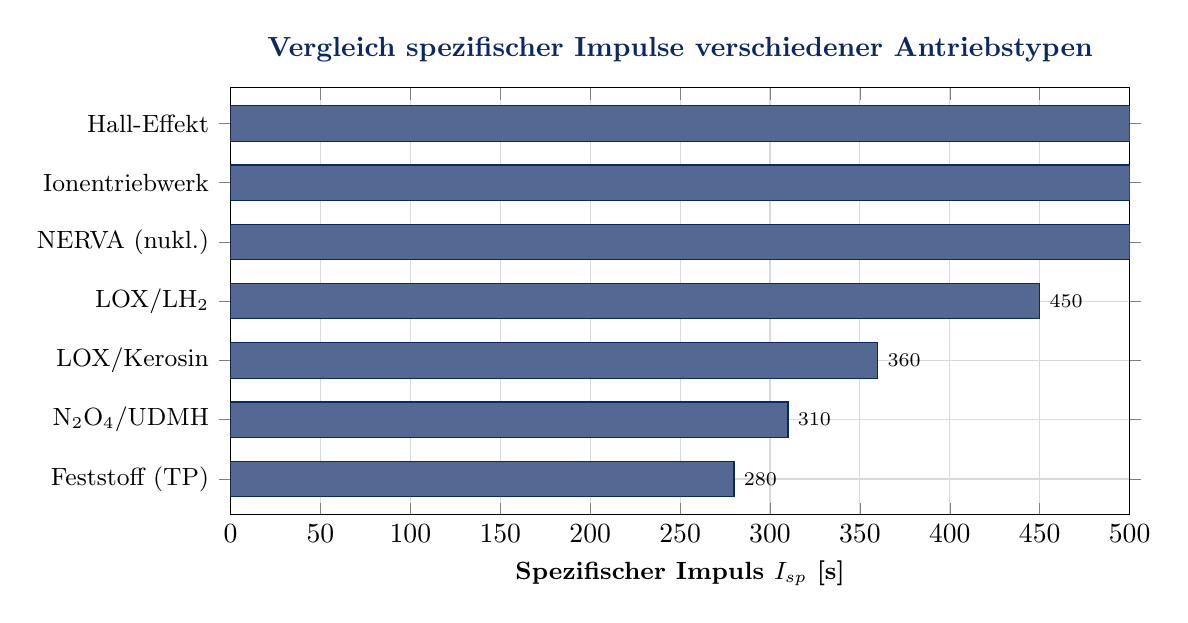
\begin{tikzpicture}
\begin{axis}[
  width=13cm, height=7cm,
  xbar, xmin=0, xmax=500,
  symbolic y coords={
    {Feststoff (TP)},
    {N$_2$O$_4$/UDMH},
    {LOX/Kerosin},
    {LOX/LH$_2$},
    {NERVA (nukl.)},
    {Ionentriebwerk},
    {Hall-Effekt}},
  ytick=data,
  xlabel={Spezifischer Impuls $I_{sp}$ [s]},
  xlabel style={font=\small\bfseries},
  yticklabel style={font=\small},
  title={Vergleich spezifischer Impulse verschiedener Antriebstypen},
  title style={font=\normalsize\bfseries\color{raumblau}},
  bar width=0.45cm,
  nodes near coords,
  nodes near coords align={horizontal},
  every node near coord/.style={font=\scriptsize},
  grid=major,
  grid style={draw=gray!30},
]
\addplot[fill=raumblau!70, draw=raumblau] coordinates {
  (280,{Feststoff (TP)})
  (310,{N$_2$O$_4$/UDMH})
  (360,{LOX/Kerosin})
  (450,{LOX/LH$_2$})
  (800,{NERVA (nukl.)})
  (3000,{Ionentriebwerk})
  (1500,{Hall-Effekt})
};
\end{axis}
\end{tikzpicture}
\caption{Spezifische Impulse $\Isp$ typischer Antriebskonzepte. Elektrische Antriebe
(Ionen, Hall-Effekt) erzielen zwar hohe $\Isp$-Werte, erzeugen aber nur sehr geringe
Schubkräfte ($\ll \SI{1}{N}$).}
\label{fig:isp_vergleich}
\end{figure}

%=======================================================
\section{Chemische Raketentriebwerke}
%=======================================================

\subsection{Flüssigkeits-Raketentriebwerk (LRE)}

Ein Flüssigraketentriebwerk (engl. \emph{Liquid Rocket Engine}, LRE) verbrennt
flüssige Treibstoffe --- meist Brennstoff (Fuel) und Oxidator (Oxidizer) getrennt ---
in einer Brennkammer bei hohem Druck ($p_c = 5\ldots\SI{250}{bar}$).

\begin{figure}[H]
\centering
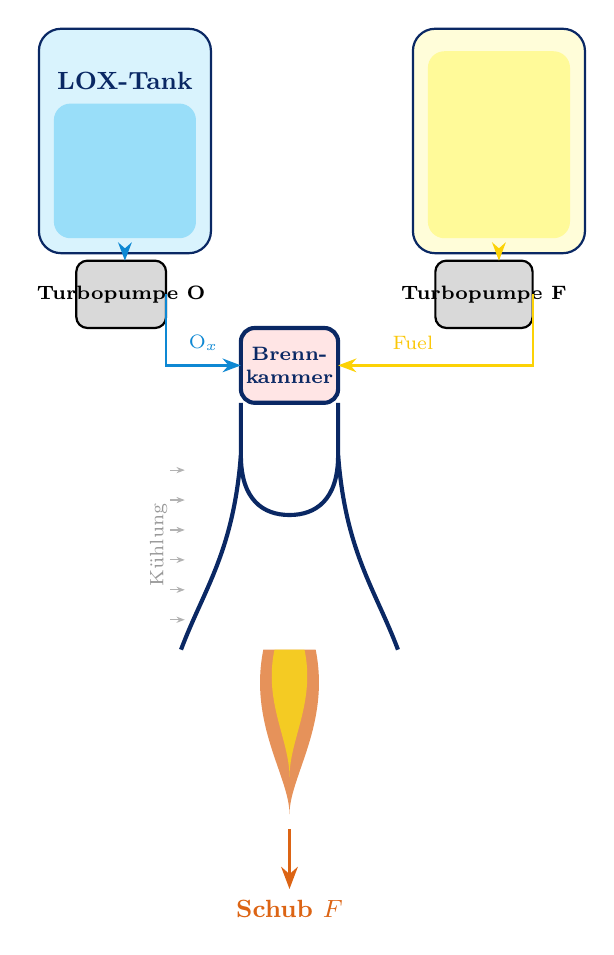
\begin{tikzpicture}[scale=0.95]
  % ---- Tanks ----
  % LOX-Tank (links)
  \draw[thick, raumblau, fill=cyan!15, rounded corners=8pt]
    (-5.5, 1.5) rectangle (-3.2, 4.5);
  \node[font=\small\bfseries, raumblau] at (-4.35, 3.8) {LOX-Tank};
  \node[font=\scriptsize] at (-4.35, 3.1) {flüssiger};
  \node[font=\scriptsize] at (-4.35, 2.7) {Sauerstoff};
  \node[font=\scriptsize] at (-4.35, 2.2) {$T=-183\,°C$};
  % Füllstand
  \fill[cyan!40, rounded corners=6pt]
    (-5.3,1.7) rectangle (-3.4,3.5);

  % LH2-Tank (rechts)
  \draw[thick, raumblau, fill=yellow!15, rounded corners=8pt]
    (-0.5, 1.5) rectangle (1.8, 4.5);
  \node[font=\small\bfseries, raumblau] at (0.65, 3.8) {LH$_2$-Tank};
  \node[font=\scriptsize] at (0.65, 3.1) {flüssiger};
  \node[font=\scriptsize] at (0.65, 2.7) {Wasserstoff};
  \node[font=\scriptsize] at (0.65, 2.2) {$T=-253\,°C$};
  \fill[yellow!40, rounded corners=6pt]
    (-0.3,1.7) rectangle (1.6,4.2);

  % Turbopumpen
  \draw[thick, fill=gray!30, rounded corners=4pt]
    (-5.0,0.5) rectangle (-3.8,1.4);
  \node[font=\scriptsize\bfseries] at (-4.4,0.95) {Turbopumpe O};

  \draw[thick, fill=gray!30, rounded corners=4pt]
    (-0.2,0.5) rectangle (1.1,1.4);
  \node[font=\scriptsize\bfseries] at (0.45,0.95) {Turbopumpe F};

  % Leitungen Tank -> Turbopumpe
  \draw[thick, cyan!70!blue, -{Stealth}]
    (-4.35,1.5) -- (-4.35,1.4);
  \draw[thick, yellow!70!orange, -{Stealth}]
    (0.65,1.5) -- (0.65,1.4);

  % Brennkammer
  \draw[thick, raumblau, line width=1.5pt, fill=red!10, rounded corners=5pt]
    (-2.8,-0.5) rectangle (-1.5,0.5);
  \node[font=\scriptsize\bfseries, raumblau] at (-2.15,0.15) {Brenn-};
  \node[font=\scriptsize\bfseries, raumblau] at (-2.15,-0.15) {kammer};

  % Einspritzung
  \draw[thick, cyan!70!blue, -{Stealth}]
    (-3.8,0.95) -- (-3.8,0.0) -- (-2.8,0.0);
  \draw[thick, yellow!70!orange, -{Stealth}]
    (1.1,0.95) -- (1.1,0.0) -- (-1.5,0.0);

  % Leitungsbeschriftung
  \node[font=\scriptsize, cyan!70!blue] at (-3.3,0.3) {O$_x$};
  \node[font=\scriptsize, yellow!60!orange] at (-0.5,0.3) {Fuel};

  % Lavaldüse
  \draw[thick, raumblau, line width=1.5pt]
    (-2.8,-0.5) -- (-2.8,-1.2) .. controls (-2.8,-1.8) and (-2.5,-2.0) ..
    (-2.15,-2.0) .. controls (-1.8,-2.0) and (-1.5,-1.8) ..
    (-1.5,-1.2) -- (-1.5,-0.5);

  % Divergenter Teil
  \draw[thick, raumblau, line width=1.5pt]
    (-2.8,-1.2) .. controls (-2.9,-2.5) and (-3.3,-3.0) ..
    (-3.6,-3.8);
  \draw[thick, raumblau, line width=1.5pt]
    (-1.5,-1.2) .. controls (-1.4,-2.5) and (-1.0,-3.0) ..
    (-0.7,-3.8);

  % Flamme
  \fill[triebwerkorange, opacity=0.7]
    (-2.5,-3.8) .. controls (-2.7,-4.8) and (-2.15,-5.5) .. (-2.15,-6.0)
    .. controls (-2.15,-5.5) and (-1.6,-4.8) .. (-1.8,-3.8) -- cycle;
  \fill[yellow, opacity=0.6]
    (-2.35,-3.8) .. controls (-2.5,-4.5) and (-2.15,-5.0) .. (-2.15,-5.5)
    .. controls (-2.15,-5.0) and (-1.8,-4.5) .. (-1.95,-3.8) -- cycle;

  % Schub-Pfeil
  \draw[-{Stealth[length=8pt, width=6pt]}, very thick, triebwerkorange]
    (-2.15,-6.2) -- (-2.15,-7.0) node[below, font=\small\bfseries] {Schub $F$};

  % Regenerativkühlung (Pfeile an Düsenwand)
  \foreach \y in {-1.4,-1.8,-2.2,-2.6,-3.0,-3.4} {
    \draw[-{Stealth[length=3pt]}, gray!60, line width=0.4pt]
      (-3.75,\y) -- (-3.55,\y);
  }
  \node[font=\scriptsize, gray!80, rotate=90] at (-3.9,-2.4) {Kühlung};
\end{tikzpicture}
\caption{Schematischer Aufbau eines kryogenen Flüssig-Raketentriebwerks (LOX/LH$_2$).
Beide Treibstoffkomponenten werden durch Turbopumpen in die Brennkammer gefördert,
dort verbrannt und durch die Lavaldüse expandiert.}
\label{fig:lre}
\end{figure}

\subsection{Verbrennungstemperatur und Heizwert}

Die Verbrennungstemperatur $T_c$ beeinflusst $v_e$ maßgeblich. Für die Reaktion
von Wasserstoff mit Sauerstoff:
\[
  \mathrm{2\,H_2 + O_2 \longrightarrow 2\,H_2O},\quad
  \Delta H_R = -\SI{483.6}{kJ/mol}
\]
Die adiabate Flammentemperatur ergibt sich aus der Wärmebilanz:
\[
  \sum_i n_i\,c_{p,i}\,(T_c - T_{\text{ref}}) = -\Delta H_R
  \quad\Rightarrow\quad T_c \approx \SI{3500}{K}
\]

\subsection{Schubkammerauslegung --- Kenngrößen}

\begin{table}[H]
\centering
\caption{Auslegungsgrößen für ein typisches LOX/LH$_2$-Triebwerk (Vakuumbetrieb)}
\label{tab:triebwerk}
\begin{tabular}{lrrl}
\toprule
\textbf{Größe} & \textbf{Symbol} & \textbf{Wert} & \textbf{Einheit}\\
\midrule
Brennkammerdruck        & $p_c$     & 200        & bar\\
Brennkammertemperatur   & $T_c$     & 3500       & K\\
Düsenhalsdurchmesser    & $d^*$     & 0.20       & m\\
Expansionsverhältnis    & $\varepsilon = A_e/A^*$ & 77.5 & --\\
Isentropenexponent      & $\gamma$  & 1.26       & --\\
Molare Masse Abgas      & $\bar{M}$ & 10.0       & g/mol\\
Massenfluss             & $\mdot$   & 500        & kg/s\\
Spezifischer Impuls     & $\Isp$    & 451        & s\\
Vakuumschub             & $F_{\mathrm{vac}}$ & 2200 & kN\\
\bottomrule
\end{tabular}
\end{table}

\textbf{Berechnung des Ausströmimpulses:}
\begin{align}
  v_e &= \sqrt{\frac{2\gamma}{\gamma-1}\cdot\frac{R\,T_c}{\bar{M}}
    \left[1 - \left(\frac{p_e}{p_c}\right)^{(\gamma-1)/\gamma}\right]} \notag\\
  &= \sqrt{\frac{2\times1{,}26}{0{,}26}\cdot\frac{8{,}314\times3500}{0{,}010}
    \left[1 - \left(\frac{0{,}002}{200}\right)^{0{,}26/1{,}26}\right]} \notag\\
  &\approx \SI{4\,420}{m/s}
\end{align}

%=======================================================
\section{Elektrische Antriebe}
%=======================================================

Elektrische Antriebe beschleunigen das Treibmittel nicht durch chemische Verbrennung,
sondern durch elektrische oder elektromagnetische Felder. Sie erzielen weit höhere
Ausströmgeschwindigkeiten ($v_e = 20\ldots\SI{200}{km/s}$), haben aber sehr geringe
Massenflüsse und damit extrem kleine Schubkräfte.

\subsection{Ionentriebwerk (Gitterionen-Triebwerk)}

\begin{figure}[H]
\centering
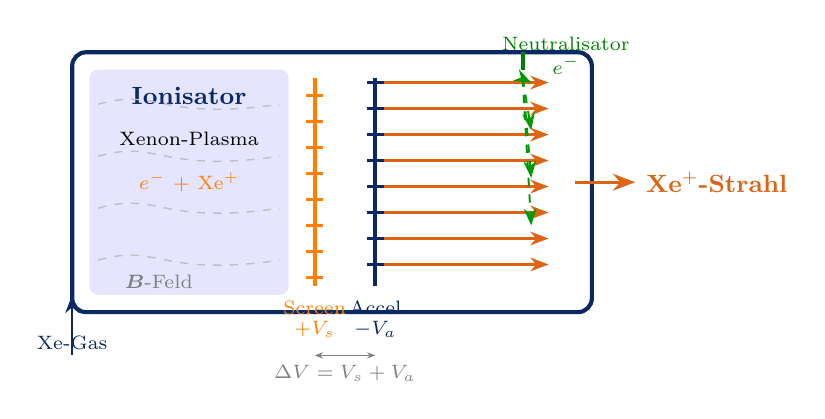
\begin{tikzpicture}[scale=1.1]
  % Gehäuse
  \draw[thick, raumblau, line width=1.5pt, rounded corners=5pt]
    (0,0) rectangle (6,3);

  % Ionisationszone
  \fill[blue!10, rounded corners=3pt] (0.2,0.2) rectangle (2.5,2.8);
  \node[font=\small\bfseries, raumblau] at (1.35,2.5) {Ionisator};
  \node[font=\scriptsize] at (1.35,2.0) {Xenon-Plasma};
  \node[font=\scriptsize, orange] at (1.35,1.5) {$e^-$ + Xe$^+$};

  % Magnetfeldlinien (Darstellung)
  \foreach \y in {0.6,1.2,1.8,2.4} {
    \draw[gray!50, dashed, line width=0.5pt]
      (0.3,\y) .. controls (1.0,\y+0.2) and (1.0,\y-0.2) .. (2.4,\y);
  }
  \node[font=\scriptsize, gray] at (1.0,0.35) {$\vek{B}$-Feld};

  % Gitter 1 (Schirm-Gitter)
  \draw[thick, orange, line width=1.5pt] (2.8,0.3) -- (2.8,2.7);
  \foreach \y in {0.4,0.7,1.0,1.3,1.6,1.9,2.2,2.5} {
    \draw[orange, line width=1pt] (2.7,\y) -- (2.9,\y);
  }
  \node[font=\scriptsize, orange] at (2.8,0.05) {Screen};
  \node[font=\scriptsize, orange] at (2.8,-0.2) {$+V_s$};

  % Gitter 2 (Beschleunigungs-Gitter)
  \draw[thick, raumblau, line width=1.5pt] (3.5,0.3) -- (3.5,2.7);
  \foreach \y in {0.55,0.85,1.15,1.45,1.75,2.05,2.35,2.65} {
    \draw[raumblau, line width=1pt] (3.4,\y) -- (3.6,\y);
  }
  \node[font=\scriptsize, raumblau] at (3.5,0.05) {Accel};
  \node[font=\scriptsize, raumblau] at (3.5,-0.2) {$-V_a$};

  % Ionenstrahlen
  \foreach \y in {0.55,0.85,1.15,1.45,1.75,2.05,2.35,2.65} {
    \draw[-{Stealth}, triebwerkorange, line width=0.8pt]
      (3.6,\y) -- (5.5,\y);
  }

  % Neutralisator (Elektronenstrahl)
  \draw[thick, green!50!black, line width=1.5pt]
    (5.2,3.0) -- (5.2,2.8);
  \foreach \y in {2.65,2.1,1.55,1.0} {
    \draw[-{Stealth}, green!60!black, line width=0.7pt, dashed]
      (5.2,2.7) -- (5.2+0.1,\y);
  }
  \node[font=\scriptsize, green!50!black] at (5.7,3.1) {Neutralisator};
  \node[font=\scriptsize, green!50!black] at (5.7,2.85) {$e^-$};

  % Ausströmung
  \draw[-{Stealth[length=8pt]}, very thick, triebwerkorange]
    (5.8,1.5) -- (6.5,1.5) node[right, font=\small\bfseries] {Xe$^+$-Strahl};

  % Xenon-Einlass
  \draw[-{Stealth}, thick, raumblau]
    (0,-0.5) -- (0,0.2) node[below=0.4cm, font=\scriptsize] {Xe-Gas};

  % Spannungsbezeichnung
  \draw[{Stealth[length=3pt]}-{Stealth[length=3pt]}, gray]
    (2.8,-0.5) -- (3.5,-0.5) node[midway, below, font=\scriptsize] {$\Delta V = V_s+V_a$};
\end{tikzpicture}
\caption{Gitterionen-Triebwerk (Gridded Ion Thruster). Xenon-Atome werden ionisiert,
durch ein elektrisches Gitter auf $v_e = 30\ldots\SI{90}{km/s}$ beschleunigt und
durch den Neutralisator wieder elektrisch neutralisiert.}
\label{fig:ionentriebwerk}
\end{figure}

\subsection{Energiebilanz Ionentriebwerk}

Die kinetische Energie des Ionenstrahls berechnet sich zu:
\[
  E_{\mathrm{kin}} = \frac{1}{2}\mdot\,v_e^2 = q\,\Delta V\,\dot{n}
\]
wobei $q$ die Ionenladung, $\Delta V$ die Beschleunigungsspannung und $\dot{n}$ der
Ionenstromfluss ist. Die Ausströmgeschwindigkeit ergibt sich aus:
\[
  \frac{1}{2}m_{\mathrm{Xe}}\,v_e^2 = q\,\Delta V
  \quad\Rightarrow\quad
  v_e = \sqrt{\frac{2q\,\Delta V}{m_{\mathrm{Xe}}}}
\]

Für Xenon ($m_{\mathrm{Xe}} = \SI{2.18e-25}{kg}$, $q = \SI{1.6e-19}{C}$,
$\Delta V = \SI{1200}{V}$):
\[
  v_e = \sqrt{\frac{2 \times 1{,}6\times10^{-19} \times 1200}{2{,}18\times10^{-25}}}
  \approx \SI{41\,800}{m/s} = \SI{41.8}{km/s}
\]

Der Systemwirkungsgrad (elektrische Eingangsleistung $P$ zu Strahlleistung):
\[
  \eta_T = \frac{\frac{1}{2}F\,v_e}{P}
\]

\subsection{Hall-Effekt-Triebwerk (HET)}

\begin{figure}[H]
\centering
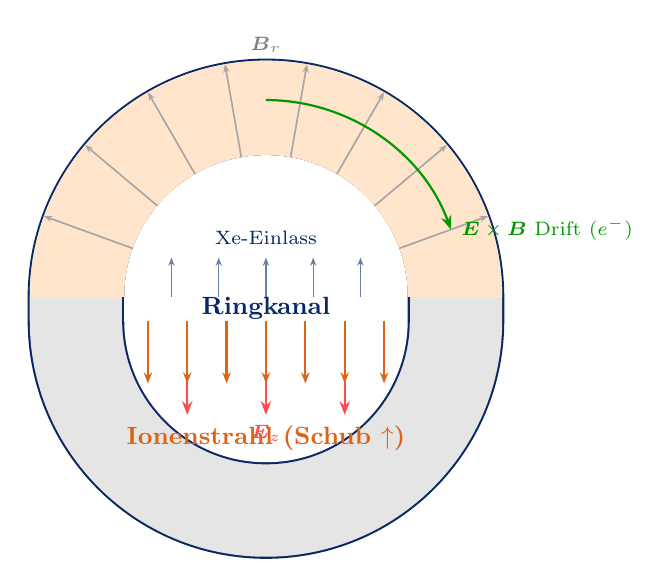
\begin{tikzpicture}[scale=1.0]
  % Ringkanal (Querschnitt)
  % Außenwand
  \draw[thick, raumblau, line width=1.5pt]
    (0,0) arc(180:0:3.0) -- (6,0) -- (6,-0.3) arc(0:-180:3.0) -- cycle;
  \fill[gray!20]
    (0,0) arc(180:0:3.0) -- (6,0) -- (6,-0.3) arc(0:-180:3.0) -- cycle;

  % Innenwand
  \draw[thick, raumblau, line width=1.5pt]
    (1.2,0) arc(180:0:1.8) -- (4.8,0) -- (4.8,-0.3) arc(0:-180:1.8) -- cycle;
  \fill[white]
    (1.2,0) arc(180:0:1.8) -- (4.8,0) -- (4.8,-0.3) arc(0:-180:1.8) -- cycle;

  % Plasmakanal (oben)
  \fill[orange!20]
    (0,0) arc(180:0:3.0) -- (6,0)
    -- (4.8,0) arc(0:180:1.8) -- cycle;

  % Magnetfeldlinien (radial)
  \foreach \angle in {20,40,60,80,100,120,140,160} {
    \pgfmathsetmacro{\xinner}{3.0 + 1.8*cos(\angle)}
    \pgfmathsetmacro{\yinner}{1.8*sin(\angle)}
    \pgfmathsetmacro{\xouter}{3.0 + 3.0*cos(\angle)}
    \pgfmathsetmacro{\youter}{3.0*sin(\angle)}
    \draw[-{Stealth[length=3pt]}, gray!70, line width=0.6pt]
      (\xinner,\yinner) -- (\xouter,\youter);
  }
  \node[font=\scriptsize, gray] at (3,3.2) {$\vek{B}_r$};

  % E-Feld (axial)
  \draw[-{Stealth[length=5pt]}, thick, red!70]
    (3.0,-0.8) -- (3.0,-1.5) node[below, font=\scriptsize, red!70] {$\vek{E}_z$};
  \draw[-{Stealth[length=5pt]}, thick, red!70]
    (2.0,-0.8) -- (2.0,-1.5);
  \draw[-{Stealth[length=5pt]}, thick, red!70]
    (4.0,-0.8) -- (4.0,-1.5);

  % Elektronendrift (azimuthal, E×B)
  \draw[-{Stealth[length=5pt]}, thick, green!60!black]
    (3.0,2.5) arc(90:20:2.5) node[right, font=\scriptsize, green!60!black]
    {$\vek{E}\times\vek{B}$ Drift ($e^-$)};

  % Ionenstrahl (axial nach unten)
  \foreach \x in {1.5, 2.0, 2.5, 3.0, 3.5, 4.0, 4.5} {
    \draw[-{Stealth[length=4pt]}, triebwerkorange, line width=0.8pt]
      (\x,-0.3) -- (\x,-1.1);
  }
  \node[font=\small\bfseries, triebwerkorange] at (3.0,-1.8)
    {Ionenstrahl (Schub $\uparrow$)};

  % Xe-Einlass
  \foreach \x in {1.8, 2.4, 3.0, 3.6, 4.2} {
    \draw[-{Stealth[length=3pt]}, raumblau!60, line width=0.5pt]
      (\x,0.0) -- (\x,0.5);
  }
  \node[font=\scriptsize, raumblau] at (3.0,0.75) {Xe-Einlass};

  % Beschriftungen
  \node[font=\small\bfseries, raumblau] at (3.0,-0.15) {Ringkanal};
\end{tikzpicture}
\caption{Querschnitt eines Hall-Effekt-Triebwerks (HET). Das radiale Magnetfeld $\vek{B}_r$
und das axiale elektrische Feld $\vek{E}_z$ zwingen Elektronen auf eine azimuthale
Driftbahn ($\vek{E}\times\vek{B}$-Drift), die Xenon-Ionen werden axial beschleunigt.}
\label{fig:het}
\end{figure}

%=======================================================
\section{Bahnmechanik und $\Delta v$-Budget}
%=======================================================

\subsection{Kreisbahngeschwindigkeit und Fluchtgeschwindigkeit}

Für einen Satelliten auf einer Kreisbahn im Radius $r$ um die Erde gilt
Kräftegleichgewicht zwischen Gravitationskraft und Zentripetalkraft:

\[
  \frac{GMm}{r^2} = \frac{mv_c^2}{r}
  \quad\Rightarrow\quad
  v_c(r) = \sqrt{\frac{GM}{r}}
\]

\begin{table}[H]
\centering
\caption{Kreisbahngeschwindigkeiten bei verschiedenen Erdumlaufbahnen}
\label{tab:bahnen}
\begin{tabular}{lrrrr}
\toprule
\textbf{Bahn} & \textbf{Höhe [km]} & \textbf{$r$ [km]} & \textbf{$v_c$ [km/s]} & \textbf{Umlaufzeit}\\
\midrule
LEO      & 400    & 6778   & 7.67 & 92.5 min\\
MEO      & 20\,200 & 26\,578 & 3.87 & 12.0 h\\
GEO      & 35\,786 & 42\,164 & 3.07 & 24.0 h\\
Mond     & 385\,000 & 391\,378 & 1.01 & 27.3 d\\
\bottomrule
\end{tabular}
\end{table}

Die \textbf{Fluchtgeschwindigkeit} ist die Mindestgeschwindigkeit zum Verlassen des
Gravitationsfeldes (Gesamtenergie = 0):
\[
  v_{\mathrm{esc}}(r) = \sqrt{\frac{2GM}{r}} = \sqrt{2}\,v_c(r)
  \approx \SI{11.19}{km/s} \quad (r = R_\oplus)
\]

\subsection{Hohmann-Transfer}

Der \textbf{Hohmann-Transfer} ist die energieoptimale Transferbahn zwischen zwei
koplanaren Kreisbahnen.

\begin{figure}[H]
\centering
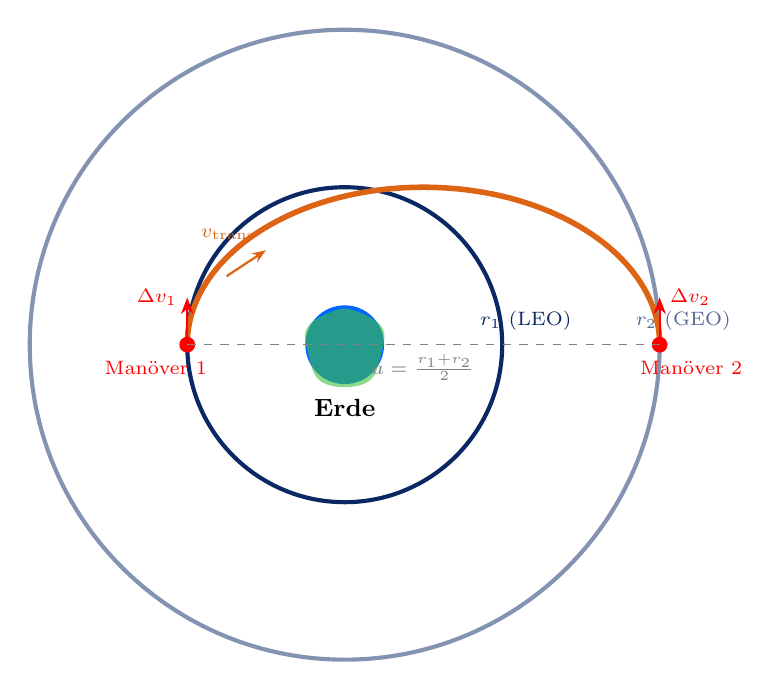
\begin{tikzpicture}[scale=1.0]
  % Erde
  \fill[blue!60!cyan] (0,0) circle (0.5cm);
  \fill[green!50!gray, opacity=0.6]
    plot[smooth, samples=50, domain=0:360]
    ({0.5*cos(\x)+0.08*cos(3*\x)*sin(\x)},{0.5*sin(\x)+0.04*cos(2*\x)});
  \node[font=\small\bfseries] at (0,-0.8) {Erde};

  % Innere Bahn (LEO)
  \draw[thick, raumblau, line width=1.5pt] (0,0) circle (2.0cm);
  \node[font=\scriptsize, raumblau] at (2.3,0.3) {$r_1$ (LEO)};

  % Äußere Bahn (GEO)
  \draw[thick, raumblau!50, line width=1.5pt] (0,0) circle (4.0cm);
  \node[font=\scriptsize, raumblau!70] at (4.3,0.3) {$r_2$ (GEO)};

  % Transfer-Ellipse (Hohmann)
  \draw[thick, triebwerkorange, line width=2pt]
    (-2,0) arc(180:0:3cm and 2cm);

  % Manöver 1 (Periapsis)
  \fill[red] (-2.0,0) circle (0.1cm);
  \draw[-{Stealth[length=6pt]}, thick, red]
    (-2.0,0) -- (-2.0,0.6) node[left, font=\scriptsize\bfseries, red]
    {$\Dv_1$};
  \node[font=\scriptsize, red] at (-2.4,-0.3) {Manöver~1};

  % Manöver 2 (Apoapsis)
  \fill[red] (4.0,0) circle (0.1cm);
  \draw[-{Stealth[length=6pt]}, thick, red]
    (4.0,0) -- (4.0,0.6) node[right, font=\scriptsize\bfseries, red]
    {$\Dv_2$};
  \node[font=\scriptsize, red] at (4.4,-0.3) {Manöver~2};

  % Geschwindigkeitspfeile auf Transferellipse
  \draw[-{Stealth[length=5pt]}, triebwerkorange, thick]
    (-1.5, 0.87) -- (-1.0, 1.2)
    node[above left, font=\scriptsize, triebwerkorange] {$v_{\mathrm{trans}}$};

  % Halbachsen
  \draw[dashed, gray] (-2,0) -- (4,0) node[midway, below, font=\scriptsize, gray]
    {$a = \frac{r_1+r_2}{2}$};
\end{tikzpicture}
\caption{Hohmann-Transfer zwischen niedrigem Erdorbit (LEO, $r_1$) und
geostationärem Orbit (GEO, $r_2$). Die Transferellipse hat ihre
Periapsis bei $r_1$ und Apoapsis bei $r_2$. Es werden zwei Impulsmanöver benötigt.}
\label{fig:hohmann}
\end{figure}

\begin{herleitung}[Hohmann-Transfer-$\Dv$]
Die große Halbachse der Transferellipse:
\[
  a_t = \frac{r_1 + r_2}{2}
\]
Aus dem Virialsatz (Vis-Viva-Gleichung):
\[
  v^2 = GM\left(\frac{2}{r} - \frac{1}{a}\right)
\]
Perigäumsgeschwindigkeit der Transferellipse:
\[
  v_{\mathrm{peri}} = \sqrt{GM\left(\frac{2}{r_1} - \frac{1}{a_t}\right)}
  = \sqrt{\frac{GM}{r_1}\cdot\frac{2r_2}{r_1+r_2}}
\]
Apogäumsgeschwindigkeit:
\[
  v_{\mathrm{apo}} = \sqrt{GM\left(\frac{2}{r_2} - \frac{1}{a_t}\right)}
  = \sqrt{\frac{GM}{r_2}\cdot\frac{2r_1}{r_1+r_2}}
\]
Gesamt-$\Dv$:
\[
  \boxed{\Dv_{\mathrm{total}} = \Dv_1 + \Dv_2
    = \left(v_{\mathrm{peri}} - v_{c,1}\right)
    + \left(v_{c,2} - v_{\mathrm{apo}}\right)}
\]
Für LEO ($r_1 = \SI{6778}{km}$) $\to$ GEO ($r_2 = \SI{42164}{km}$):
\begin{align*}
  v_{c,1} &= \sqrt{GM/r_1} = \SI{7.67}{km/s}\\
  v_{c,2} &= \sqrt{GM/r_2} = \SI{3.07}{km/s}\\
  v_{\mathrm{peri}} &= \sqrt{\frac{GM}{r_1}\cdot\frac{2r_2}{r_1+r_2}}
    = \SI{10.15}{km/s}\\
  v_{\mathrm{apo}} &= \sqrt{\frac{GM}{r_2}\cdot\frac{2r_1}{r_1+r_2}}
    = \SI{1.60}{km/s}\\
  \Dv_{\mathrm{total}} &= (10{,}15 - 7{,}67) + (3{,}07 - 1{,}60)
    = 2{,}48 + 1{,}47 = \SI{3.95}{km/s}
\end{align*}
\end{herleitung}

\subsection{Gesamtes $\Dv$-Budget einer Mondmission}

\begin{table}[H]
\centering
\caption{Typisches $\Dv$-Budget für eine Mondmission (Low-Thrust vernachlässigt)}
\label{tab:dv_mond}
\begin{tabular}{lrl}
\toprule
\textbf{Manöver} & \textbf{$\Dv$ [m/s]} & \textbf{Bemerkung}\\
\midrule
Gravity losses (Startphase)       & 1\,500 & Gravitationsverluste beim Start\\
Aerodynamischer Widerstand        &   135  & Atmosphäre ($\leq 120$ km)\\
LEO-Einschwingen                  &   100  & Kreisbahnkorrektur\\
Trans-Lunar Injection (TLI)       & 3\,130 & Verlassen der Erdumlaufbahn\\
Lunar Orbit Insertion (LOI)       &   900  & Einschuss Mondorbit\\
Powered Descent                   & 1\,900 & Mondlandung\\
Mondstart + Rendezvous            & 1\,850 & Aufstieg + Andocken\\
Trans-Earth Injection (TEI)       &   850  & Rückkehr Erde\\
\midrule
\textbf{Gesamt}                   & \textbf{10\,365} & \\
\bottomrule
\end{tabular}
\end{table}

\subsection{Stufung --- Mehrere Raketenstufen}

Da das Massenverhältnis durch Strukturmasse begrenzt ist, verwendet man \emph{mehrstufige}
Raketen. Der Gesamtgewinn durch $n$ Stufen:
\[
  \Dv_{\mathrm{ges}} = \sum_{k=1}^{n} v_{e,k}\,\ln\!\left(\frac{m_{0,k}}{m_{1,k}}\right)
\]

\begin{figure}[H]
\centering
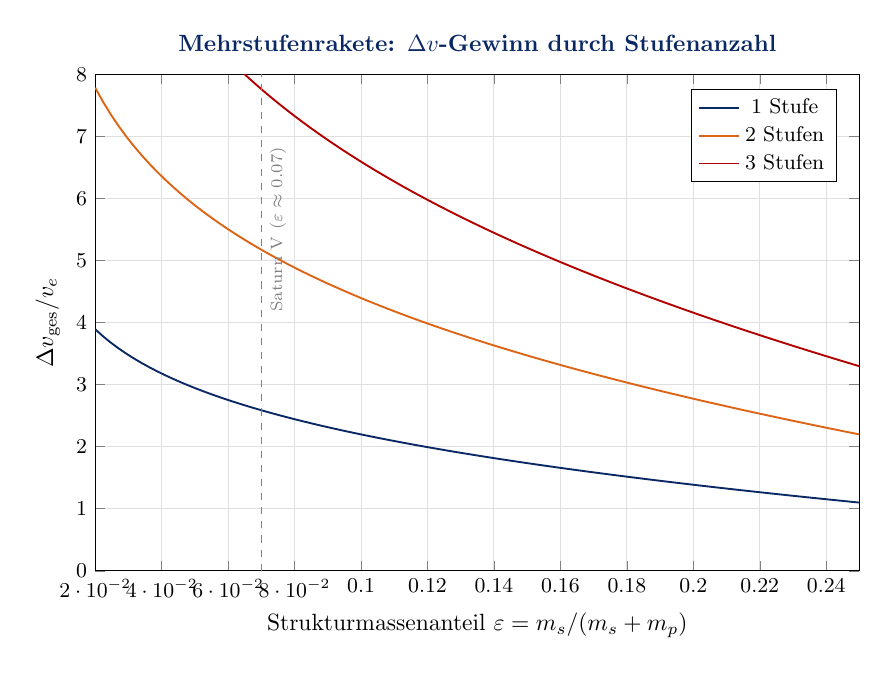
\begin{tikzpicture}[scale=0.85]
  \begin{axis}[
    width=13cm, height=9cm,
    xlabel={Strukturmassenanteil $\varepsilon = m_s/(m_s+m_p)$},
    ylabel={$\Dv_{\mathrm{ges}}/v_e$},
    xmin=0.02, xmax=0.25,
    ymin=0, ymax=8,
    grid=both,
    grid style={draw=gray!25},
    title={Mehrstufenrakete: $\Dv$-Gewinn durch Stufenanzahl},
    title style={font=\normalsize\bfseries\color{raumblau}},
    legend pos=north east,
    legend style={font=\small},
    tick label style={font=\small},
  ]
  % 1 Stufe
  \addplot[thick, raumblau, domain=0.02:0.25, samples=100]
    {ln((1-x)/x)};
  \addlegendentry{1 Stufe}
  % 2 Stufen
  \addplot[thick, triebwerkorange, domain=0.02:0.25, samples=100]
    {2*ln((1-x)/x)};
  \addlegendentry{2 Stufen}
  % 3 Stufen
  \addplot[thick, red!70!black, domain=0.02:0.25, samples=100]
    {3*ln((1-x)/x)};
  \addlegendentry{3 Stufen}
  % Typischer Strukturanteil Saturn V
  \addplot[dashed, gray, domain=0:8] coordinates {(0.07,0)(0.07,8)};
  \node[font=\scriptsize, gray, rotate=90] at (axis cs:0.075,5.5)
    {Saturn~V $(\varepsilon\approx0.07)$};
  \end{axis}
\end{tikzpicture}
\caption{Gewinn durch Stufenanzahl: Bei einem typischen Strukturanteil $\varepsilon$ mit $\varepsilon = 0.07$
und $v_e = \SI{4.4}{km/s}$ ermöglicht eine dreistufige Rakete
$\Dv \approx 3 \times \ln(13.3) \times 4.4 \approx \SI{33}{km/s}$ --- deutlich mehr
als für eine Mondmission benötigt.}
\label{fig:stufen}
\end{figure}

%=======================================================
\section{Nuklearer Raketenantrieb}
%=======================================================

\subsection{Kernthermal-Antrieb (NTR)}

Beim Kernthermal-Antrieb (engl. \emph{Nuclear Thermal Rocket}, NTR) wird Wasserstoff
als Treibmittel durch einen Kernreaktor auf $T \approx 2500\ldots\SI{3000}{K}$ erhitzt
und durch eine Düse expandiert. Der Reaktor erzeugt keinerlei chemische Energie ---
der Wasserstoff verbrennt nicht, er wird nur erhitzt.

Da nur Wasserstoff ($\bar{M} = \SI{2}{g/mol}$) ausgestoßen wird, ergibt sich ein
sehr hoher spezifischer Impuls:

\[
  v_e \propto \sqrt{\frac{T}{\bar{M}}}
  \quad\Rightarrow\quad
  \Isp^{\mathrm{NTR}} \approx 800\ldots\SI{900}{s}
\]

\begin{figure}[H]
\centering
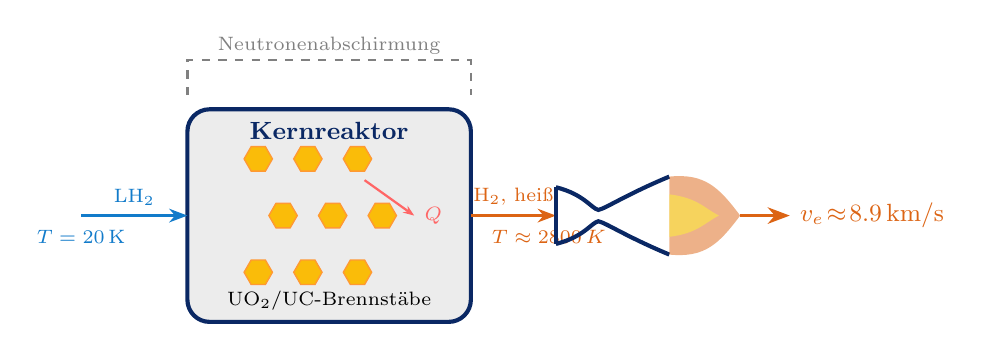
\begin{tikzpicture}[scale=0.9]
  % Reaktor
  \draw[thick, raumblau, line width=1.5pt, rounded corners=8pt, fill=gray!15]
    (-2.0, -1.5) rectangle (2.0, 1.5);

  % Reaktorkern (hexagonal representation)
  \foreach \x in {-1.0,-0.3,0.4} {
    \foreach \y in {-0.8,-0.0,0.8} {
      \pgfmathsetmacro{\xo}{\x + 0.35*(mod(int((\y+0.8)/0.8), 2))}
      \draw[fill=yellow!50!orange, draw=orange!80, line width=0.5pt]
        (\xo,\y) +(0:0.2) \foreach \a in {60,120,180,240,300,360} {-- +(\a:0.2)} -- cycle;
    }
  }
  \node[font=\small\bfseries, raumblau] at (0,1.2) {Kernreaktor};
  \node[font=\scriptsize] at (0,-1.2) {UO$_2$/UC-Brennstäbe};

  % H2-Einlass (links)
  \draw[thick, cyan!60!blue, -{Stealth}]
    (-3.5,0) -- (-2.0,0) node[midway, above, font=\scriptsize] {LH$_2$};
  \node[font=\scriptsize, cyan!60!blue] at (-3.5,-0.3) {$T=\SI{20}{K}$};

  % Erhitzter H2-Auslass (rechts -> Düse)
  \draw[thick, triebwerkorange, -{Stealth}]
    (2.0,0) -- (3.2,0) node[midway, above, font=\scriptsize] {H$_2$, heiß};
  \node[font=\scriptsize, triebwerkorange] at (3.1,-0.3) {$T\approx2800\,K$};

  % Düse (konvergent-divergent)
  \draw[thick, raumblau, line width=1.5pt]
    (3.2,0.4) -- (3.2,-0.4);
  \draw[thick, raumblau, line width=1.5pt]
    (3.2,0.4) .. controls (3.6,0.3) and (3.7,0.1) ..
    (3.8,0.08) .. controls (3.9,0.1) and (4.2,0.3) .. (4.8,0.55);
  \draw[thick, raumblau, line width=1.5pt]
    (3.2,-0.4) .. controls (3.6,-0.3) and (3.7,-0.1) ..
    (3.8,-0.08) .. controls (3.9,-0.1) and (4.2,-0.3) .. (4.8,-0.55);

  % Abgasstrahl
  \fill[triebwerkorange, opacity=0.5]
    (4.8,0.55) .. controls (5.3,0.6) and (5.5,0.4) .. (5.8,0.0)
    .. controls (5.5,-0.4) and (5.3,-0.6) .. (4.8,-0.55) -- cycle;
  \fill[yellow!80, opacity=0.5]
    (4.8,0.3) .. controls (5.2,0.25) and (5.3,0.1) .. (5.5,0.0)
    .. controls (5.3,-0.1) and (5.2,-0.25) .. (4.8,-0.3) -- cycle;

  \draw[-{Stealth[length=8pt]}, thick, triebwerkorange]
    (5.8,0) -- (6.5,0) node[right, font=\small\bfseries] {$v_e\!\approx\!\SI{8.9}{km/s}$};

  % Neutronenabsorber
  \draw[thick, gray, dashed]
    (-2.0,1.7) -- (-2.0,2.2) -- (2.0,2.2) -- (2.0,1.7);
  \node[font=\scriptsize, gray] at (0,2.4) {Neutronenabschirmung};

  % Wärmepfeil
  \draw[-{Stealth[length=4pt]}, red!60, line width=0.8pt]
    (0.5,0.5) -- (1.2,0.0) node[right, font=\scriptsize, red!60] {$Q$};
\end{tikzpicture}
\caption{Kernthermal-Raketenantrieb (NTR). Flüssiger Wasserstoff wird durch den Reaktor
auf $\sim\SI{2800}{K}$ erhitzt und durch die Düse expandiert. Es findet \emph{keine}
Verbrennung statt --- der Reaktor liefert nur Wärme. $\Isp \approx \SI{850}{s}$.}
\label{fig:ntr}
\end{figure}

%=======================================================
\section{Vergleichende Zusammenfassung}
%=======================================================

\begin{figure}[H]
\centering
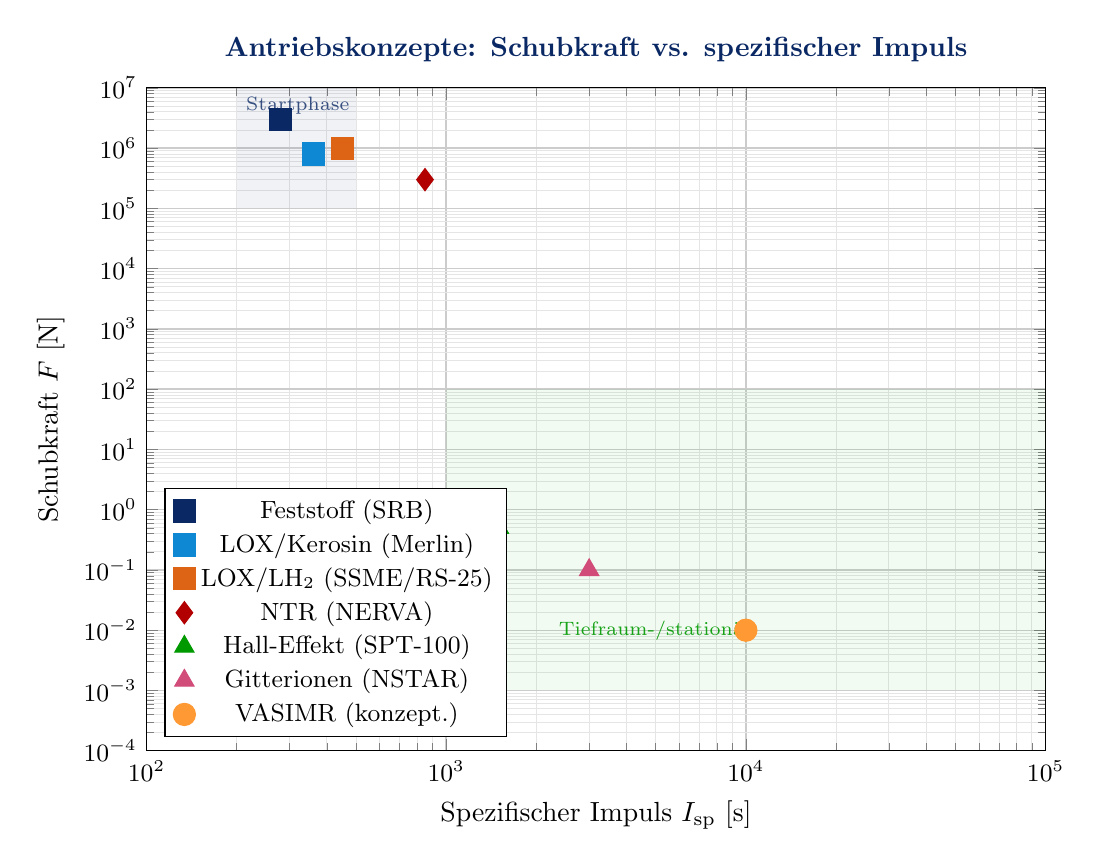
\begin{tikzpicture}
\begin{loglogaxis}[
  width=13cm, height=10cm,
  xlabel={Spezifischer Impuls $\Isp$ [s]},
  ylabel={Schubkraft $F$ [N]},
  xmin=100, xmax=100000,
  ymin=0.0001, ymax=10000000,
  grid=both,
  grid style={draw=gray!20, line width=0.3pt},
  major grid style={draw=gray!40, line width=0.5pt},
  title={Antriebskonzepte: Schubkraft vs. spezifischer Impuls},
  title style={font=\normalsize\bfseries\color{raumblau}},
  legend style={font=\small, at={(0.02,0.02)}, anchor=south west},
  tick label style={font=\small},
]
% Datenpunkte (Mitte der typischen Bereiche)
\addplot[only marks, mark=square*, mark size=4pt, color=raumblau]
  coordinates {(280, 3e6)};
\addlegendentry{Feststoff (SRB)}

\addplot[only marks, mark=square*, mark size=4pt, color=cyan!70!blue]
  coordinates {(360, 8e5)};
\addlegendentry{LOX/Kerosin (Merlin)}

\addplot[only marks, mark=square*, mark size=4pt, color=triebwerkorange]
  coordinates {(451, 1e6)};
\addlegendentry{LOX/LH$_2$ (SSME/RS-25)}

\addplot[only marks, mark=diamond*, mark size=4pt, color=red!70!black]
  coordinates {(850, 3e5)};
\addlegendentry{NTR (NERVA)}

\addplot[only marks, mark=triangle*, mark size=4pt, color=green!60!black]
  coordinates {(1500, 0.5)};
\addlegendentry{Hall-Effekt (SPT-100)}

\addplot[only marks, mark=triangle*, mark size=4pt, color=purple!70]
  coordinates {(3000, 0.1)};
\addlegendentry{Gitterionen (NSTAR)}

\addplot[only marks, mark=*, mark size=4pt, color=orange!80]
  coordinates {(10000, 0.01)};
\addlegendentry{VASIMR (konzept.)}

% Nutzungsregionen
\fill[raumblau, opacity=0.06]
  (axis cs:200,1e5) rectangle (axis cs:500,1e7);
\node[font=\scriptsize, raumblau, opacity=0.8] at (axis cs:320,5e6)
  {Startphase};

\fill[green!70!black, opacity=0.05]
  (axis cs:1000,0.001) rectangle (axis cs:100000,100);
\node[font=\scriptsize, green!60!black, opacity=0.9] at (axis cs:5000,0.01)
  {Tiefraum-/stationär};
\end{loglogaxis}
\end{tikzpicture}
\caption{Vergleich aller Antriebskonzepte in der Schubkraft-$\Isp$-Ebene
(doppellogarithmisch). Chemische Triebwerke liefern hohen Schub für die Startphase,
elektrische Antriebe hohen $\Isp$ für Tiefraummissionen --- ein fundamentaler Kompromiss.}
\label{fig:vergleich}
\end{figure}

\begin{table}[H]
\centering
\caption{Übersicht aller behandelten Antriebskonzepte}
\label{tab:uebersicht}
\begin{tabular}{lrrll}
\toprule
\textbf{Antrieb} & \textbf{$\Isp$ [s]} & \textbf{$F$ [N]} &
\textbf{Treibmittel} & \textbf{Anwendung}\\
\midrule
Feststoff (SRB)   & 250--280  & $10^5\ldots10^7$ & APCP     & Booster, Start\\
LOX/Kerosin       & 300--360  & $10^4\ldots10^6$ & RP-1/LOX & 1. Stufe\\
LOX/LH$_2$        & 420--460  & $10^4\ldots10^6$ & LH$_2$/LOX& 2./3. Stufe\\
N$_2$O$_4$/UDMH   & 300--320  & $10^3\ldots10^5$ & Hypergol & OMS, RCS\\
NTR (nuklear)     & 800--900  & $10^4\ldots10^5$ & LH$_2$   & Marsreise\\
Hall-Effekt (HET) & 1000--2000 & $0.05\ldots5$   & Xenon    & GEO-Antrieb\\
Gitterionen       & 2000--5000 & $0.001\ldots0.5$& Xenon    & Tiefraumsonde\\
VASIMR            & 3000--30000& $0.005\ldots10$ & Plasma   & konzept.\\
\bottomrule
\end{tabular}
\end{table}

%=======================================================
\section{Schlussbetrachtung}
%=======================================================

Die Entwicklung von Raketenantrieben ist untrennbar mit zwei fundamentalen Spannungsfeldern
verbunden: dem \emph{Schub-$\Isp$-Kompromiss} und der \emph{Treibstoffmassentyrannei}
der Tsiolkowski-Gleichung.

Chemische Triebwerke bleiben für die Startphase alternativlos, weil sie die einzige
Technologie darstellen, die Schubkräfte von mehreren Meganewton bei ausreichend hohem
$\Isp$ vereint. Die kinetische Energie des Raumfahrzeugs beim Erreichen der
Kreisbahngeschwindigkeit ($\frac{1}{2}mv_c^2 = \frac{1}{2}m\cdot(7670)^2 \approx
\SI{29.5}{MJ/kg}$) entspricht exakt dem chemischen Energiepotenzial hochwertiger
Treibstoffe.

Für Missionen jenseits der Erdumlaufbahn --- Mond, Mars, äußeres Sonnensystem ---
gewinnt der spezifische Impuls zunehmend an Bedeutung. Ein Hall-Effekt-Triebwerk
mit $\Isp = \SI{1500}{s}$ benötigt für dasselbe $\Dv$ nur ein Massenverhältnis von
$m_0/m_1 = e^{\Dv/(g_0\cdot\Isp)}$, was die benötigte Treibstoffmasse dramatisch
reduziert --- der Preis ist jedoch die sehr geringe Schubkraft und damit lange
Manöverdauer.

Kernthermische Antriebe ($\Isp \approx 850$ s) stellen eine vielversprechende Brücke dar:
Sie übertreffen chemische Systeme um etwa den Faktor~2 im $\Isp$, bei noch nutzbaren
Schubkräften. Das NASA-Programm DRACO testet derartige Systeme als Kandidaten für
bemannte Marsreisen.

Die Zukunft liegt in der optimalen Kombination aller Konzepte: chemischer Hochschub
für den Start, elektrische Hocheffizienzantriebe für interplanetare Cruise-Phasen,
und möglicherweise Fusions- oder Antimaterie-Antriebe für interstellare Distanzen ---
jenseits des gegenwärtigen Technologiestands, aber innerhalb der Physik.

\bigskip
\paragraph*{Kernaussagen}
\begin{itemize}[leftmargin=*]
  \item Die \textbf{Tsiolkowski-Gleichung} $\Dv = v_e\ln(m_0/m_1)$ ist das
    fundamentale Designgesetz jeder Rakete.
  \item Die \textbf{Lavaldüse} wandelt thermische Energie isentrop in gerichteten
    Impuls --- die de Laval-Kontraktion erzwingt Überschallströmung.
  \item Chemische Triebwerke: $\Isp = 250\ldots460$ s --- optimal für \textbf{Schub}.
  \item Elektrische Antriebe: $\Isp = 1000\ldots30000$ s --- optimal für \textbf{Effizienz}.
  \item Der \textbf{Hohmann-Transfer} ist das energieoptimale Manöver zwischen
    koplanaren Kreisbahnen: $\Dv_{\mathrm{LEO\to GEO}} \approx \SI{3.95}{km/s}$.
  \item \textbf{Mehrstufige Raketen} überwinden die Massentyrannei durch sukzessives
    Abwerfen leerer Strukturmasse.
\end{itemize}

%=======================================================
\begin{thebibliography}{9}
%=======================================================

\bibitem{tsiolkovsky1903}
K.\,E. Tsiolkovsky:
\textit{Investigation of Outer Space Rocket Devices}.
Nauchnoe Obozrenie (Science Review), 1903.

\bibitem{sutton2017}
G.\,P. Sutton, O. Biblarz:
\textit{Rocket Propulsion Elements}.
9.\,Aufl. Wiley, Hoboken, 2017.

\bibitem{turner2009}
M.\,J.\,L. Turner:
\textit{Rocket and Spacecraft Propulsion -- Principles, Practice and New Developments}.
3.\,Aufl. Springer, Berlin, 2009.

\bibitem{curtis2014}
H.\,D. Curtis:
\textit{Orbital Mechanics for Engineering Students}.
3.\,Aufl. Butterworth-Heinemann, Oxford, 2014.

\bibitem{braeuning2015}
W.\,J.\,G. Bräunling:
\textit{Flugzeugtriebwerke -- Grundlagen, Aero-Thermodynamik, ideale und reale Kreisprozesse}.
4.\,Aufl. Springer, Berlin, 2015.

\bibitem{wertz2011}
J.\,R. Wertz, D.\,F. Everett, J.\,J. Puschell (Hrsg.):
\textit{Space Mission Engineering: The New SMAD}.
Microcosm Press, Hawthorne, 2011.

\end{thebibliography}

\end{document}
